\section{Bipartition}
\label{chp:bipartition}

Die Besonderheit eines bipartiten Graphen ist die Unterteilung aller Knoten in zwei disjunkte Mengen, wobei innerhalb beider Mengen keine Kanten existieren. Knoten dürfen dementsprechend nur miteinander verbunden sein, falls sich diese nicht in derselben Menge befinden. Allen nicht bipartiten Graphen fehlt es an solch einer Eigenschaft. \cite{ohlbach2018graphen}

\begin{figure}
    \centering
    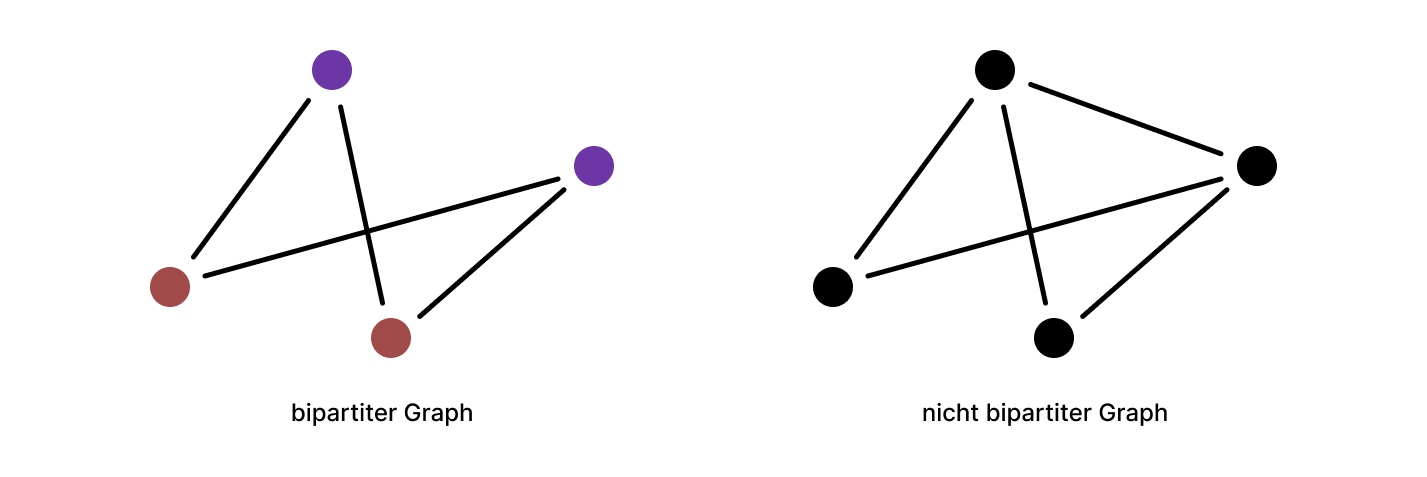
\includegraphics[width=1\textwidth]{content/img/Research/Graphen/Bipartition.png}
    \caption{Graph, welcher zwei Mengen ohne inhärente Verbindungen hat (links); keine Bipartition möglich beim rechten Graph}
    \label{fig:bipartition}
\end{figure}
\FloatBarrier